\documentclass[tikz,border=12pt]{standalone}
\usepackage{fontspec}
\setmainfont{Segoe UI}
\usepackage{amsmath,amssymb}
\usepackage{tikz}

\usetikzlibrary{calc,arrows.meta}

\begin{document}
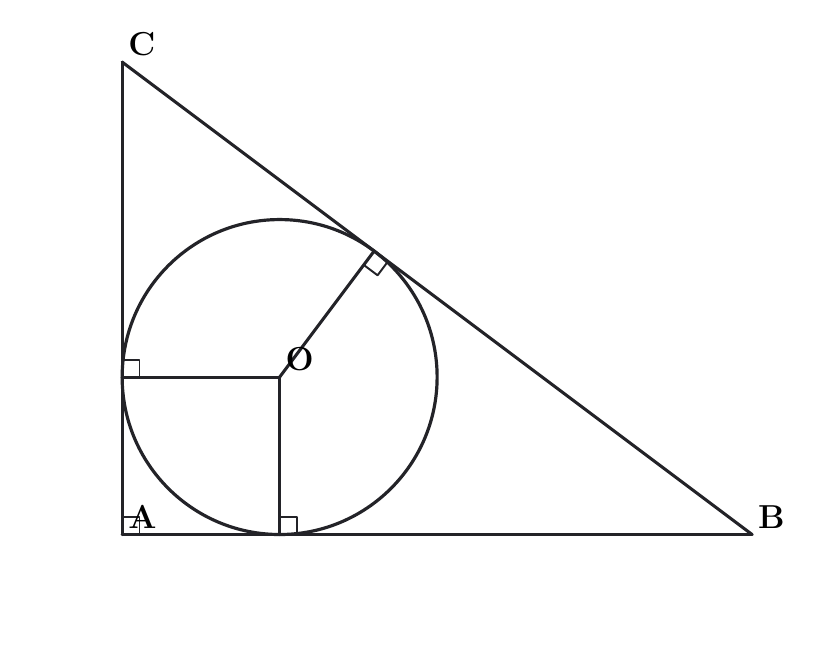
\begin{tikzpicture}[x=1.0000cm,y=1cm,line cap=round,line join=round]
\definecolor{linec0}{RGB}{35,35,40}
\definecolor{linec1}{RGB}{35,35,40}
\definecolor{linec2}{RGB}{35,35,40}
\definecolor{linec3}{RGB}{35,35,40}
\definecolor{linec4}{RGB}{35,35,40}
\definecolor{linec5}{RGB}{35,35,40}
\definecolor{edgecol}{RGB}{35,35,40}
\definecolor{hicol}{RGB}{35,35,40}
\definecolor{angcol}{RGB}{35,35,40}
\coordinate (A) at (0.0000,0.0000);
\coordinate (B) at (8.0000,0.0000);
\coordinate (C) at (0.0000,6.0000);
\coordinate (O) at (2.0000,2.0000);
\coordinate (X) at (2.0000,0.0000);
\coordinate (Y) at (0.0000,2.0000);
\coordinate (Z) at (3.2000,3.6000);
\draw[edgecol,line width=1.1pt] (A) -- (B);
\draw[edgecol,line width=1.1pt] (B) -- (C);
\draw[edgecol,line width=1.1pt] (C) -- (A);
\draw[edgecol,line width=1.1pt] (O) -- (X);
\draw[edgecol,line width=1.1pt] (O) -- (Y);
\draw[edgecol,line width=1.1pt] (O) -- (Z);
\draw[edgecol,line width=1.15pt] (O) circle [x radius=2.0000, y radius=2.0000];
\path (-1.200,-1.200) rectangle (5.200,5.200);
\draw[edgecol,line width=0.7pt] (0.220,0.000) -- (0.220,0.220) -- (0.000,0.220);
\draw[edgecol,line width=0.7pt] (2.220,0.000) -- (2.220,0.220) -- (2.000,0.220);
\draw[edgecol,line width=0.7pt] (0.000,2.220) -- (0.220,2.220) -- (0.220,2.000);
\draw[edgecol,line width=0.7pt] (3.376,3.468) -- (3.244,3.292) -- (3.068,3.424);
\node[font=\bfseries\large,inner sep=2pt,anchor=south west] at (0.000,0.000) {A};
\node[font=\bfseries\large,inner sep=2pt,anchor=south west] at (8.000,0.000) {B};
\node[font=\bfseries\large,inner sep=2pt,anchor=south west] at (0.000,6.000) {C};
\node[font=\bfseries\large,inner sep=2pt,anchor=south west] at (2.000,2.000) {O};
\end{tikzpicture}
\end{document}
